%\documentclass[iop,revtex4]{emulateapj}% change onecolumn to iop for fancy, iop to twocolumn for manuscript
\documentclass[twocolumn]{emulateapj}% change onecolumn to iop for fancy, iop to onecolumn for manuscript
%\documentclass[12pt,preprint]{aastex}

\usepackage{graphicx}
\usepackage[caption=false]{subfig}
%\usepackage{lineno}
%\usepackage{blindtext}
%\linenumbers
%\usepackage{breqn}
\usepackage{amsmath}

\let\pwiflocal=\iffalse \let\pwifjournal=\iffalse
%From: http://arxiv.org/format/1512.00483
%\input{setup}
\usepackage{enumerate}
\usepackage{amsmath,amssymb}
\usepackage{bm}
\usepackage{color}
\usepackage[utf8]{inputenc}

%% For anyone who downloaded my source file from arxiv:
%% I stole most of this setup.tex from a paper by Peter .K.G. Williams, but I made a bunch of edits to satisfy my own needs. You might check his paper out (http://arxiv.org/abs/1409.4411) for the original source file or contact him if you have any questions, since I don't really understand how some of these things work. 
%One cool thing it does is you can define an object, just that when someone clicks on the pdf it will link to simbad. I could never quite get this to work, probably because you have to get the text exactly right and my motivation for getting it to work was not super high. 


% basic packages
\usepackage{amsmath,amssymb}
\usepackage[breaklinks,colorlinks,urlcolor=blue,citecolor=blue,linkcolor=blue]{hyperref}
\usepackage{epsfig}    
\usepackage{graphicx}    
\usepackage{lineno}
\usepackage{natbib}
\usepackage{bigints}
\usepackage[outdir=./]{epstopdf}



% font stuff
\usepackage[T1]{fontenc}
\pwifjournal\else
  \usepackage{microtype}
\fi


% emulateapj has overly conservative figure widths, I think because some
% people's figures don't have good margins. Override.
\pwifjournal\else
  \makeatletter
  \renewcommand\plotone[1]{%
    \centering \leavevmode \setlength{\plot@width}{0.95\linewidth}
    \includegraphics[width={\eps@scaling\plot@width}]{#1}%
  }%
  \makeatother
\fi


\makeatletter

\newcommand\@simpfx{http://simbad.u-strasbg.fr/simbad/sim-id?Ident=}

\newcommand\MakeObj[4][\@empty]{% [shortname]{ident}{url-escaped}{formalname}
  \pwifjournal%
    \expandafter\newcommand\csname pkgwobj@c@#2\endcsname[1]{\protect\object[#4]{##1}}%
  \else%
    \expandafter\newcommand\csname pkgwobj@c@#2\endcsname[1]{\href{\@simpfx #3}{##1}}%
  \fi%
  \expandafter\newcommand\csname pkgwobj@f#2\endcsname{#4}%
  \ifx\@empty#1%
    \expandafter\newcommand\csname pkgwobj@s#2\endcsname{#4}%
  \else%
    \expandafter\newcommand\csname pkgwobj@s#2\endcsname{#1}%
  \fi}%

\newcommand\MakeTrunc[2]{% {ident}{truncname}
  \expandafter\newcommand\csname pkgwobj@t#1\endcsname{#2}}%

\newcommand{\obj}[1]{%
  \expandafter\ifx\csname pkgwobj@c@#1\endcsname\relax%
    \textbf{[unknown object!]}%
  \else%
    \csname pkgwobj@c@#1\endcsname{\csname pkgwobj@s#1\endcsname}%
  \fi}
\newcommand{\objf}[1]{%
  \expandafter\ifx\csname pkgwobj@c@#1\endcsname\relax%
    \textbf{[unknown object!]}%
  \else%
    \csname pkgwobj@c@#1\endcsname{\csname pkgwobj@f#1\endcsname}%
  \fi}
\newcommand{\objt}[1]{%
  \expandafter\ifx\csname pkgwobj@c@#1\endcsname\relax%
    \textbf{[unknown object!]}%
  \else%
    \csname pkgwobj@c@#1\endcsname{\csname pkgwobj@t#1\endcsname}%
  \fi}

\makeatother


% Evil magic to patch natbib to only highlight the year paper refs, not the
% authors too; as seen in ApJ. From
% http://tex.stackexchange.com/questions/23227/.

\pwifjournal\else
  \usepackage{etoolbox}
  \makeatletter
  \patchcmd{\NAT@citex}
    {\@citea\NAT@hyper@{%
       \NAT@nmfmt{\NAT@nm}%
       \hyper@natlinkbreak{\NAT@aysep\NAT@spacechar}{\@citeb\@extra@b@citeb}%
       \NAT@date}}
    {\@citea\NAT@nmfmt{\NAT@nm}%
     \NAT@aysep\NAT@spacechar\NAT@hyper@{\NAT@date}}{}{}
  \patchcmd{\NAT@citex}
    {\@citea\NAT@hyper@{%
       \NAT@nmfmt{\NAT@nm}%
       \hyper@natlinkbreak{\NAT@spacechar\NAT@@open\if*#1*\else#1\NAT@spacechar\fi}%
         {\@citeb\@extra@b@citeb}%
       \NAT@date}}
    {\@citea\NAT@nmfmt{\NAT@nm}%
     \NAT@spacechar\NAT@@open\if*#1*\else#1\NAT@spacechar\fi\NAT@hyper@{\NAT@date}}
    {}{}
  \makeatother
\fi

\newcommand{\prob}{{\rm prob}}
\newcommand{\qN}{\{q_i\}_{i=1}^N}
\newcommand{\qM}{\{q_{im}\}_{i=1,m=0}^{N,M}}
\newcommand{\yN}{\{y_i\}_{i=1}^N}

\newcommand{\kms}{ \textrm{km s}^{-1} }

\newcommand{\vM}{\mathsf{M}}
\newcommand{\vD}{\mathsf{D}}
\newcommand{\vR}{\mathsf{R}}
\newcommand{\vC}{\mathsf{C}}
\newcommand{\fM}{ \vec{{\bm M}}}
\newcommand{\fMi}{M_i}
\newcommand{\fD}{ \vec{{\bm D}}}
\newcommand{\fDi}{D_i}
\newcommand{\fR}{ {\bm R}}
\newcommand{\dd}{\,{\rm d}}
\newcommand{\trans}{\mathsf{T}}
\newcommand{\teff}{T_\textrm{eff}}
\newcommand{\teffa}{T_\textrm{amb}}
\newcommand{\teffb}{T_\textrm{spot}}
\newcommand{\logg}{\log g}
\newcommand{\Z}{[{\rm Fe}/{\rm H}]}
\newcommand{\A}{[\alpha/{\rm Fe}]}
\newcommand{\vsini}{v \sin i}
\newcommand{\matern}{Mat\'{e}rn}
\newcommand{\HK}{$\textrm{H}_2$O-K2}
\newcommand{\cc}[2]{c_{#2}^{(#1)}} 

\newcommand{\flam}{f_\lambda}
\newcommand{\vt}{ {\bm \theta}}
\newcommand{\vT}{ {\bm \Theta}}
\newcommand{\vp}{ {\bm \phi}}
\newcommand{\vP}{ {\bm \Phi}}
\newcommand{\cheb}{ \vp_{\mathsf{P}}}
\newcommand{\chebi}[1]{ \vp_{\textrm{Cheb}_{#1}}}
\newcommand{\Cheb}{ \vP_{\textrm{Cheb}}}
\newcommand{\Chebi}[1]{ \vP_{\textrm{Cheb}_{\ne #1}}} 
\newcommand{\cov}{ \vp_{\mathsf{C}}}
\newcommand{\covi}[1]{ \vp_{\textrm{cov}_{#1}}} 
\newcommand{\Cov}{ \vP_{\textrm{cov}}}
\newcommand{\Covi}[1]{ \vP_{\textrm{cov}_{\ne #1}}} 

\newcommand{\allParameters}{\vT} 
\newcommand{\nuisanceParameters}{\vP} 

\newcommand{\KK}{\mathcal{K}}
\newcommand{\Kglobal}{\KK^{\textrm{G}}}
\newcommand{\Klocal}{\KK^{\textrm{L}}}

\newcommand{\Gl}{Gl\,51}
\newcommand{\PHOENIX}{{\sc Phoenix}}

% Appendix commands
\newcommand{\wg}{\mathbf{w}^\textrm{grid}}
\newcommand{\wgh}{\hat{\mathbf{w}}^\textrm{grid}}

\newcommand{\Sg}{\mathbf{\Sigma}^\textrm{grid}}


\newcommand{\todo}[1]{ \textcolor{blue}{\\TODO: #1}}
\newcommand{\comm}[1]{ \textcolor{red}{MGS: #1}}
\newcommand{\hili}[1]{ \textcolor{green}{#1}}
\newcommand{\ctext}[1]{ \textcolor{blue}{\% #1}}


%  From Peter Williams and Andy Mann again:
\newcommand{\um}{$\mu$m}


\newcommand{\iancze}{{\sc C15}}

\providecommand{\eprint}[1]{\href{http://arxiv.org/abs/#1}{#1}}
\providecommand{\adsurl}[1]{\href{#1}{ADS}}
\newcommand{\name}{LkCa 4 }
\newcommand{\project}[1]{\textsl{#1}}
%\def\vsini{$v\sin{i_*}$}


\slugcomment{In preparation}

\shorttitle{Spots on Sub-subgiants}

\shortauthors{TBD}

\bibliographystyle{yahapj}

\begin{document}

\title{Starspots on sub sub giants }

\author{TBD,\altaffilmark{1}, author list TBD}


\altaffiltext{1}{TBD}

\begin{abstract}

We measure the starspots on a sub sub giant.

\end{abstract}

\keywords{stars: fundamental parameters ---  stars: statistics}

\maketitle

\section{Introduction}\label{sec:intro}

We do not know what causes some sub-sub giants!
But now we know a little... more. Hence this paper!

%Fill in more theory here
\citet{somers15} emphasized the roll of starspots in inferring stellar ages.

\begin{itemize}
\item What is a sub-subgiant?
  \begin{itemize}
  \item What causes sub sub giant stars (Leiner et al. 2017)
  \end{itemize}
\item M67 S1063
\begin{itemize}
  \item Prototypical subsub (Geller et al. 2017)
  \item Binary orbit, SB1
\end{itemize}
\item Starspots as confounding factors
\begin{itemize}
  \item Inhibit convective efficiency (redder and bigger)
  \item Also confound observations: assign incorrect Teff
  \item This paper aims to measure the starspot coverage and temp
\end{itemize}
\item Layout of this paper
\end{itemize}

\section{Observation and data reduction}
\begin{itemize}
\item IGRINS observations
\item Ground-based photometric monitoring- ASASSN, AAVSO, ASAS
\item K2 data (Campaign 5), *stretch goal* C16
\item *stretch goal* APOGEE?
\item Gaia data (membership confirmed)
\end{itemize}

\section{Analysis}
\begin{itemize}
\item Summary and assumptions of our methods
\item K2 Superstamp(s)
\begin{itemize}
  \item K2 detrending
  \item Interpreting lightcurves
  \item Period and amplitude of lightcurve, with multi-term Lomb-Scargle + Fourier reconstruction
\end{itemize}
\item Phase folded archival V-band photometry (ASASSN+)
\subsection{IGRINS two-temperature spectral inference w/ Starfish}

We performed two-temperature probabilistic spectral decomposition on the IGRINS $H-$band spectrum.  We applied the spectral inference framework \texttt{Starfish} \citep{czekala15}, recently extended to support composite spectra comprised of mixtures of two distinct photospheric components \citep{2017ApJ...836..200G}.  Here, the two temperature components are labeled as $T_{\mathrm{spot}}$ and $T_{\mathrm{amb}}$ for the starspot and ambient photospheric emission respectively, with a filling factor $f$ defined as the ratio of collective projected surface area of the spot groups to the projected area of the star.

We employed the \texttt{PHOENIX} precomputed synthetic model grid with grid ranges of $3000 < T_{\mathrm{eff}} \; (K) < 5300 $, $3 < \log{g \;(cm/s)}  < 4 $, and $ -0.5 <  [\mathrm{Fe}/\mathrm{H}] <0.5$.  We trained the spectral emulator \citep{czekala15} on this grid range, while preserving the absolute model mean fluxes to enable accurate flux comparison between two photospheres of disparate characteristic temperatures.  This new approach offers improved accuracy over the scalar flux interpolated approach introduced in Appendix XX of \citet{2017ApJ...836..200G}, especially for such a large dynamic range in effective temperature.  The spectral emulator approach propagates the uncertainty attributable to the coarsely sampled \texttt{PHOENIX} models.

The pre-defined grid ranges place uniform priors over their domain.  Additionally, a threshold of 4500 K separated the allowed domains for the spot and ambient temperatures, yielding uniform priors $3000 < T_{\mathrm{spot}} \; (K) < 4500 $ and $4500 < T_{\mathrm{amb}} \; (K) < 5300$.

\subsubsection{MCMC convergence and posterior predictive checks}
Each IGRINS spectral order was fit independently, yielding over 20 individual sets of MCMC posteriors.  We employed \texttt{emcee} \citep{foreman13} with 5000 samples and 40 walkers, spot-checking the MCMC chains for signatures of steady-state posterior probability distributions suggestive of convergence.  Some orders did not pass our convergence criteria, usually due to poor initialization of nuissance parameters or overfitting.  These specrtral orders were removed from future analysis, yielding a total of nine spectral orders, shown in Figure \ref{fig:IGRINS_spectra3x3}.

\subsubsection{FIGURE: IGRINS Spectra}
\begin{figure*}
 \centering
 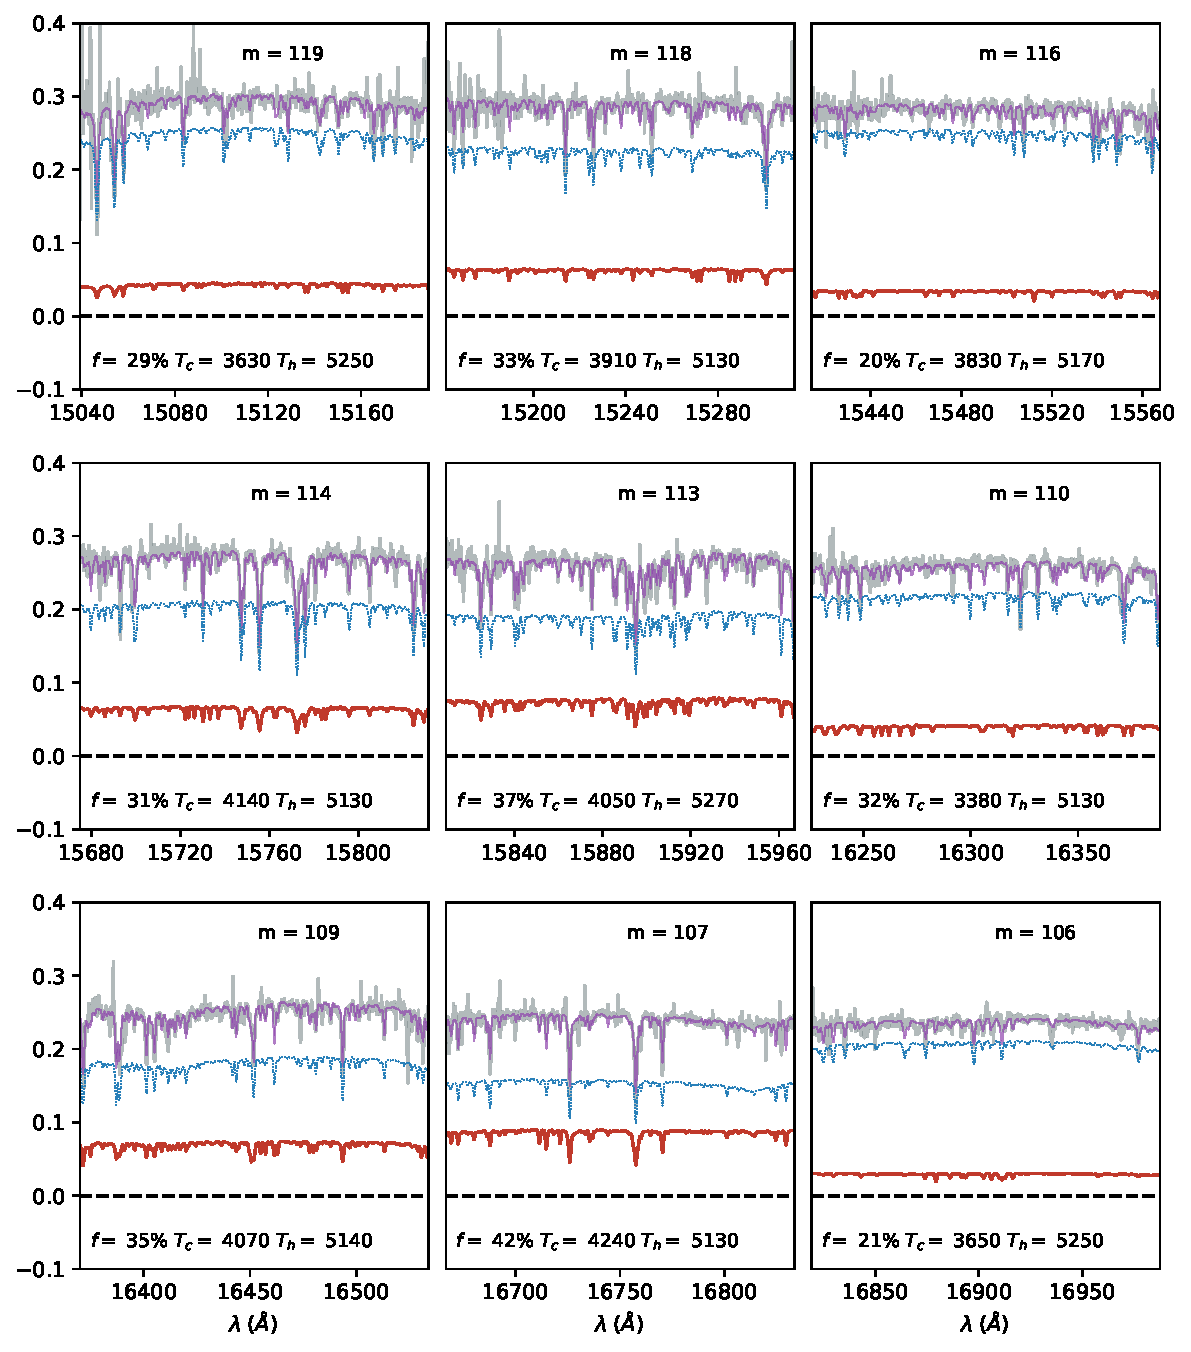
\includegraphics[width=0.98\textwidth]{figures/H_band_spectra_3x3.pdf}
 \caption{Nine $H-$band IGRINS spectral orders with probabilistic spectral decomposition.}
 \label{fig:IGRINS_spectra3x3}
\end{figure*}

\subsubsection{Internal consistency of vsini, $v_z$}
We additionally spot-checked the MCMC posteriors with posterior predictive checks... XX

\item Analysis of near-IR flux contribution from binary companion
\begin{itemize}
  \item Limits on companion types
\end{itemize}
\end{itemize}

\section{Results}

Using the \texttt{Starfish} spectral inference results we investigate the relationship between spot temperature and filling factor. In Figure XX we show 2-dimensional distributions of filling factor and spot temperature of the last 200 samples for the nine orders with accepted fits. Across the nine orders, the median filling factor value is 32\% with a standard deviation of 7\%, with a corresponding spot temperature of $4000 \pm 200$ K. The ambient photosphere temperature ssociated with this spot signature is $5200\pm25$ K. This is similar to the optical spectroscopic temperature determined by Mathieu+2003, which is expected as the optical spectrum will have less significant spot signatures than the IGRINS spectrum in the NIR.

The presence of spots impacts the effective temperature of S1063. Taking into account both temperature components, we can calculate the effective temperature using
\begin{equation}
T_{\textrm{eff}}^4 = f_{\textrm{spot}} T_{\textrm{spot}}^4 + (1 -f_{\textrm{spot}}) T_{\textrm{ambient}}^4 .
\end{equation}
This results in an updated effective temperature of 4900 K.

The IGRINS observation occurred at maximum light (LIGHT CURVE FIGURE), so this measurement of the spot filling factor is a lower limit on the total spot filling factor of S1063. We can estimate the filling factor at minimum light...

This spot coverage fraction is similar to the range of spot coverage seen on RS CVn of 30--40\% from measuring TiO band strength (O'Neal+ 1996, 98, 04) and Doppler imaging (Hackman+12). The similar spot coverage fraction on S1063 is further evidence that this sub-subgiant and likely other sub-subgiants have high magnetic activity.

\begin{itemize}
\item We detect spots in spectra
\begin{itemize}
  \item S1063 has $32 \pm 7$\% coverage fraction of spots with Tspot $4000\pm200$ K based on IGRINS + Starfish
  \item Revised effective temperature using both temperature components $[f_{\textrm{spot}} * T_{\textrm{spot}}^4 + (1 -f_{\textrm{spot}}) * T_{\textrm{ambient}}^4] = T_{\textrm{eff}}^4$

  \item *bonus* Rsini
\end{itemize}
\item IGRINS observations occurred at maximum of lightcurve, so total spot coverage is even greater
\item *bonus* total spot filling factor estimate given light curve magnitude
\item FIGURE: $T_{spot}$ versus $f_{spot}$ plot


 \begin{figure*}[h]
   \centering
   \begin{tabular}{ccc}
     \subfloat{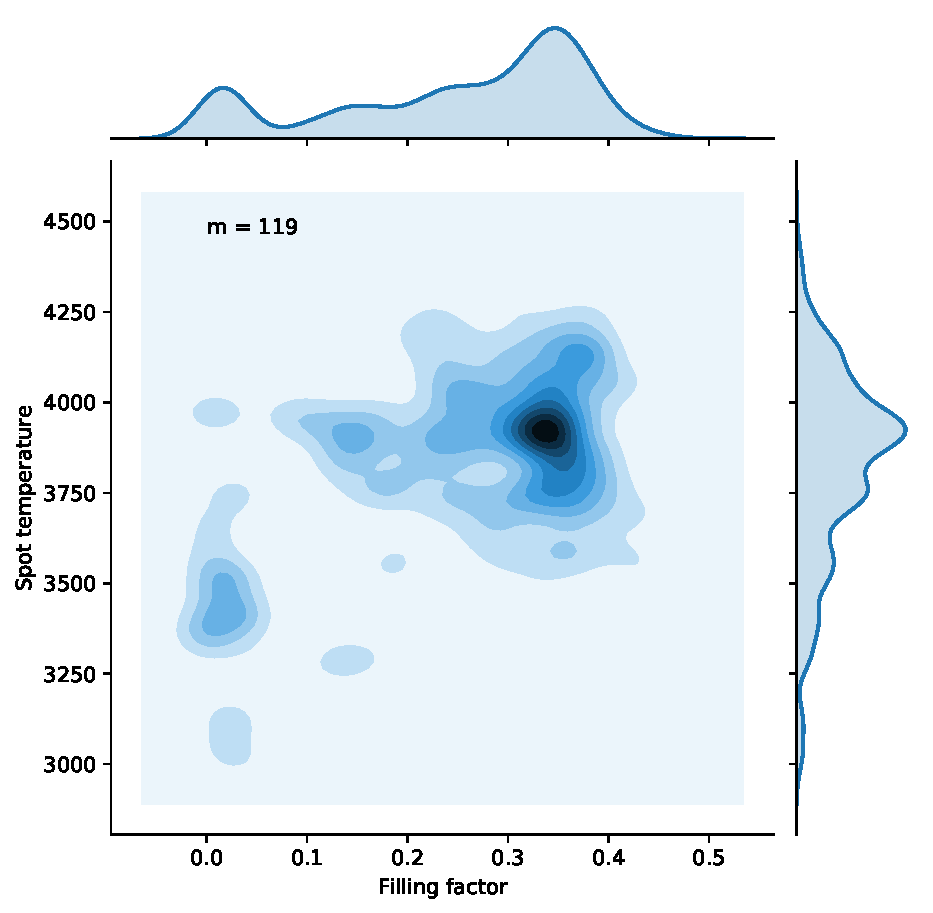
\includegraphics[width=2in]{figures/H_band_Tspot_fillingfactor_m119.pdf}} &
     \subfloat{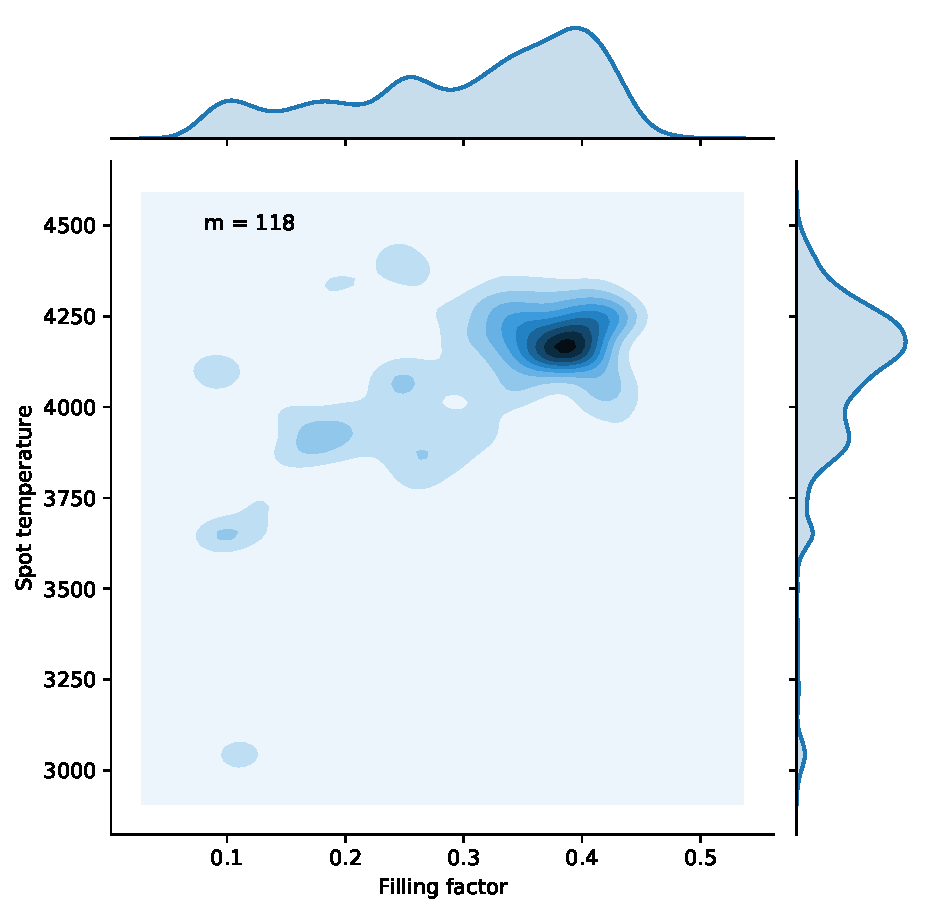
\includegraphics[width=2in]{figures/H_band_Tspot_fillingfactor_m118.pdf}} &
     \subfloat{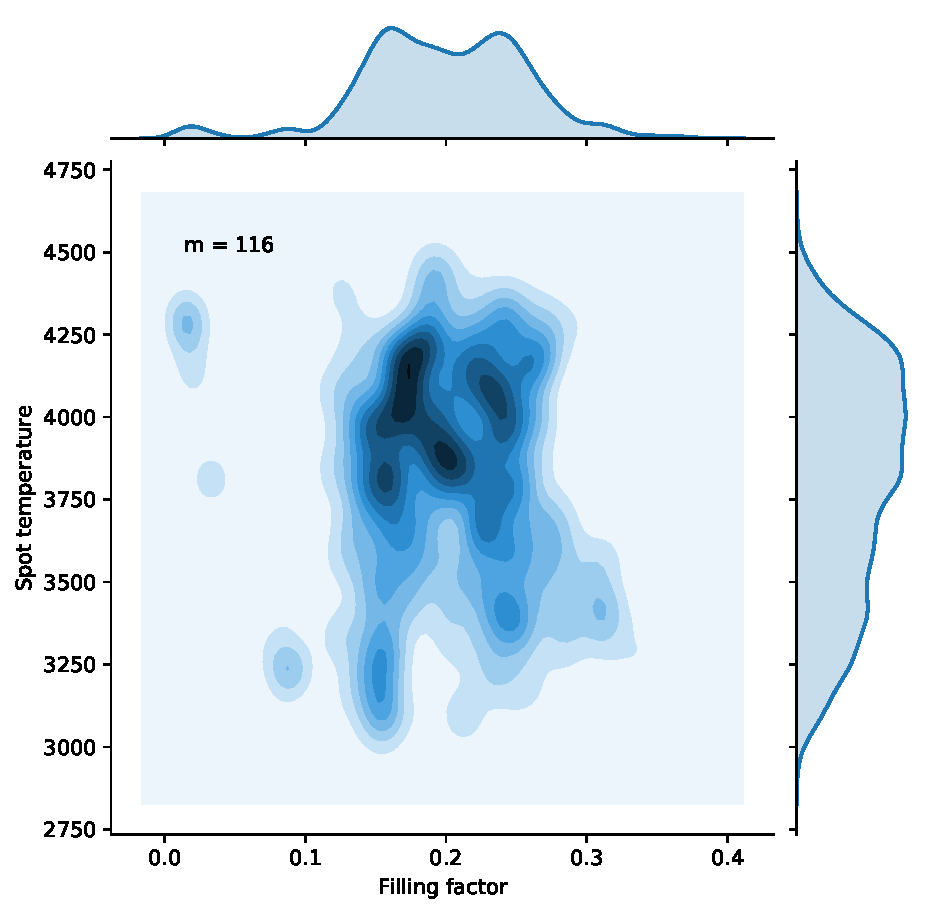
\includegraphics[width=2in]{figures/H_band_Tspot_fillingfactor_m116.pdf}} \\
     \subfloat{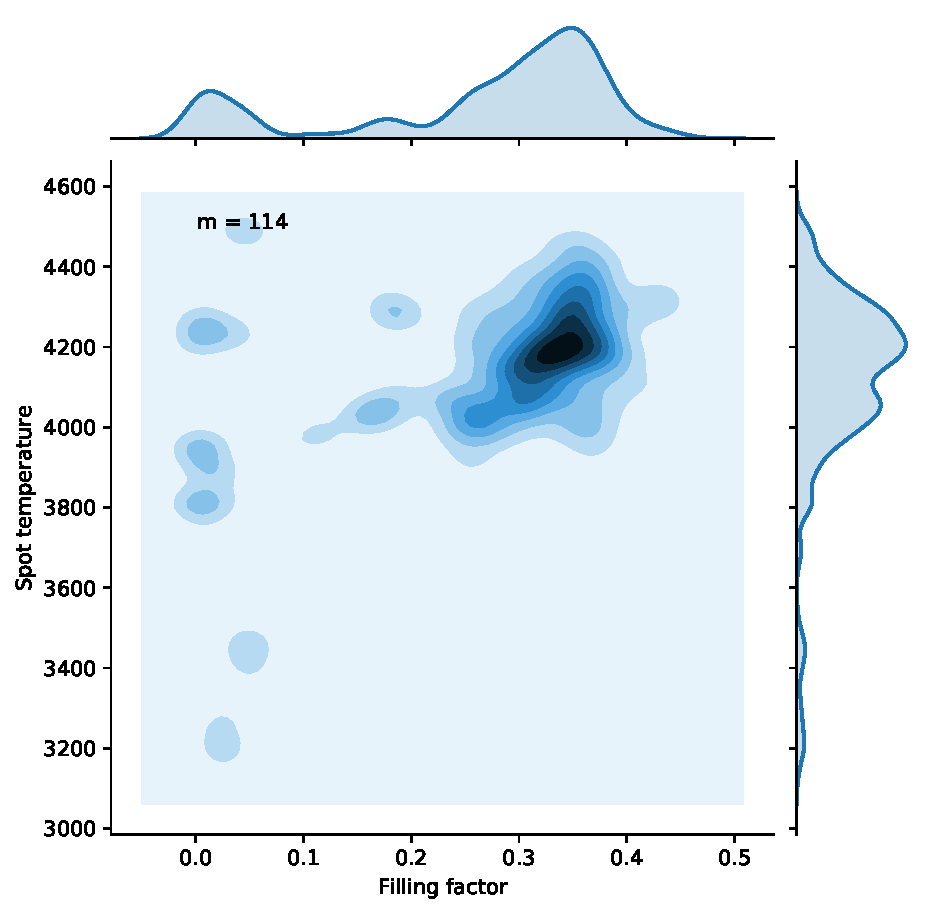
\includegraphics[width=2in]{figures/H_band_Tspot_fillingfactor_m114.pdf}} &
     \subfloat{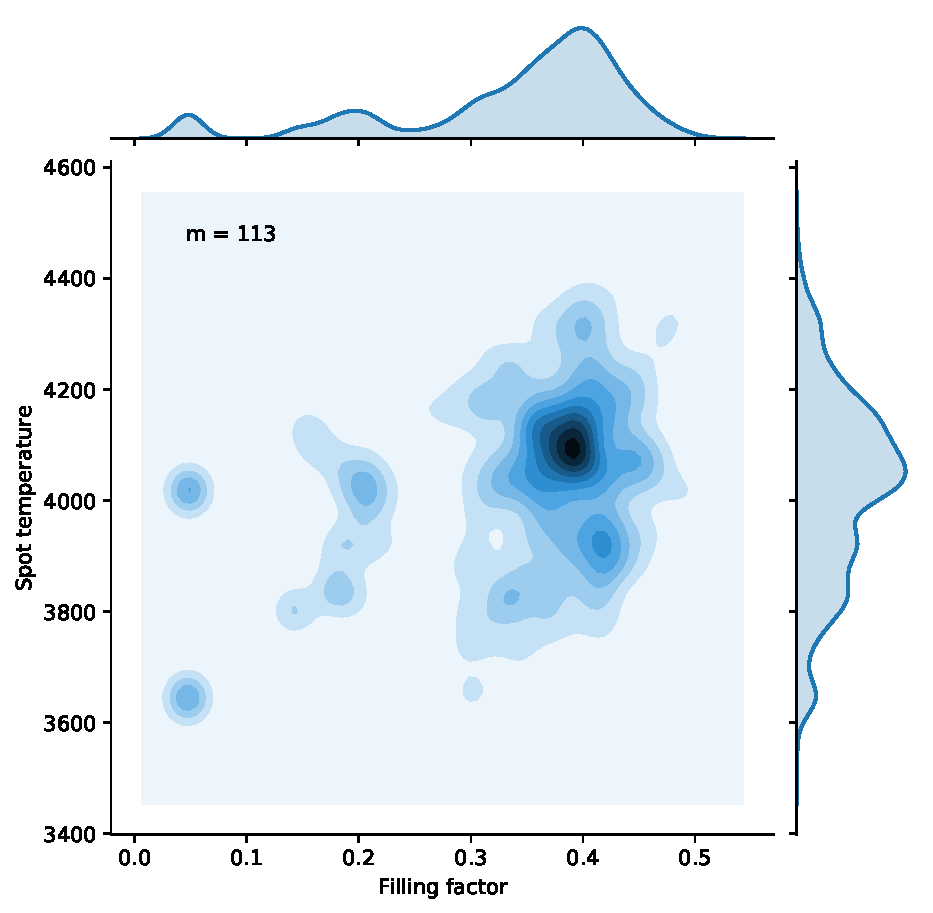
\includegraphics[width=2in]{figures/H_band_Tspot_fillingfactor_m113.pdf}} &
     \subfloat{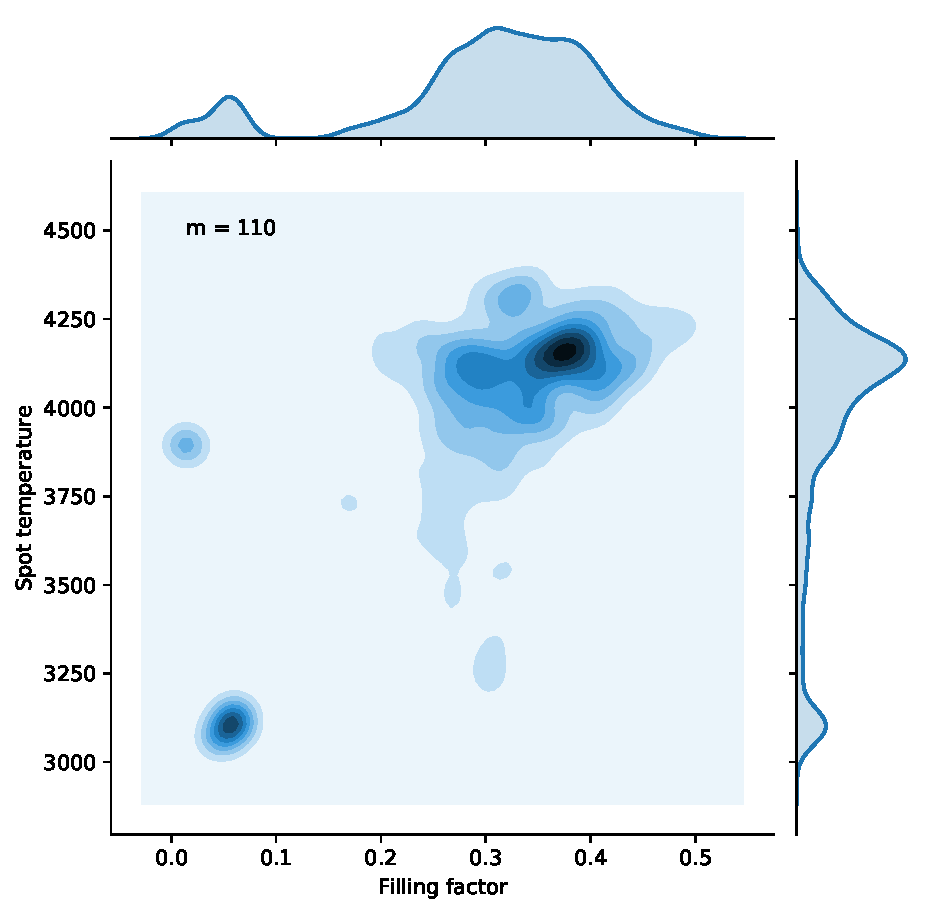
\includegraphics[width=2in]{figures/H_band_Tspot_fillingfactor_m110.pdf}} \\
     \subfloat{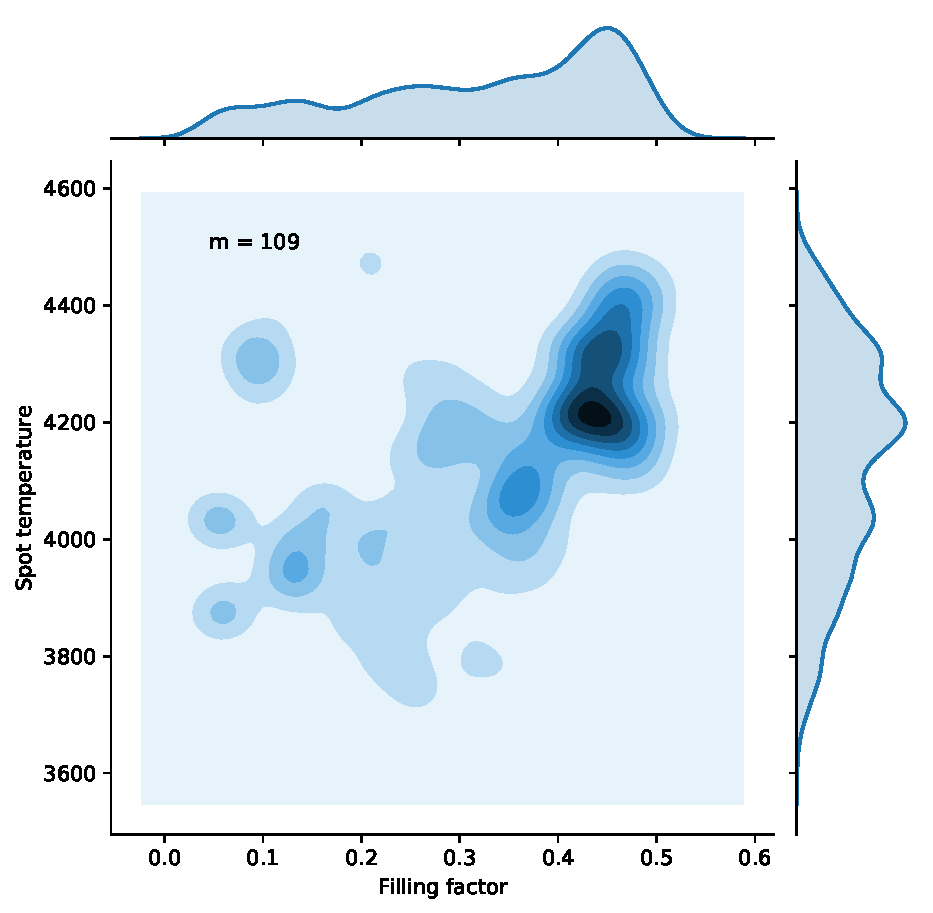
\includegraphics[width=2in]{figures/H_band_Tspot_fillingfactor_m109.pdf}} &
     \subfloat{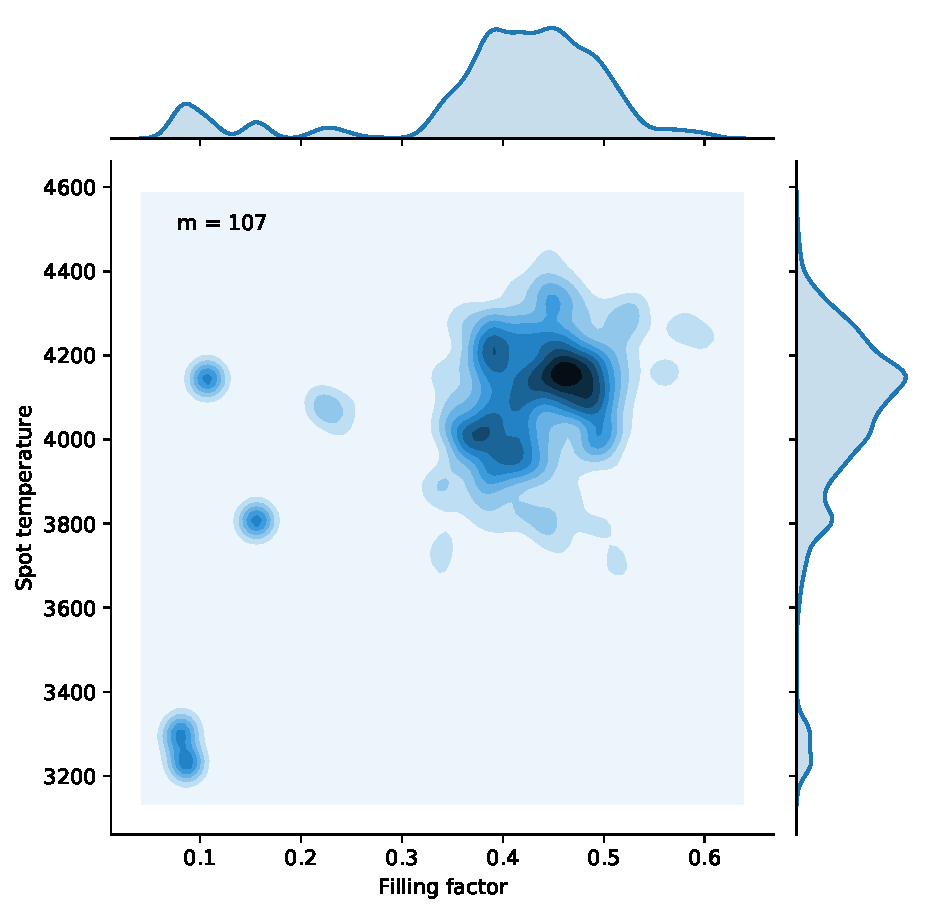
\includegraphics[width=2in]{figures/H_band_Tspot_fillingfactor_m107.pdf}} &
     \subfloat{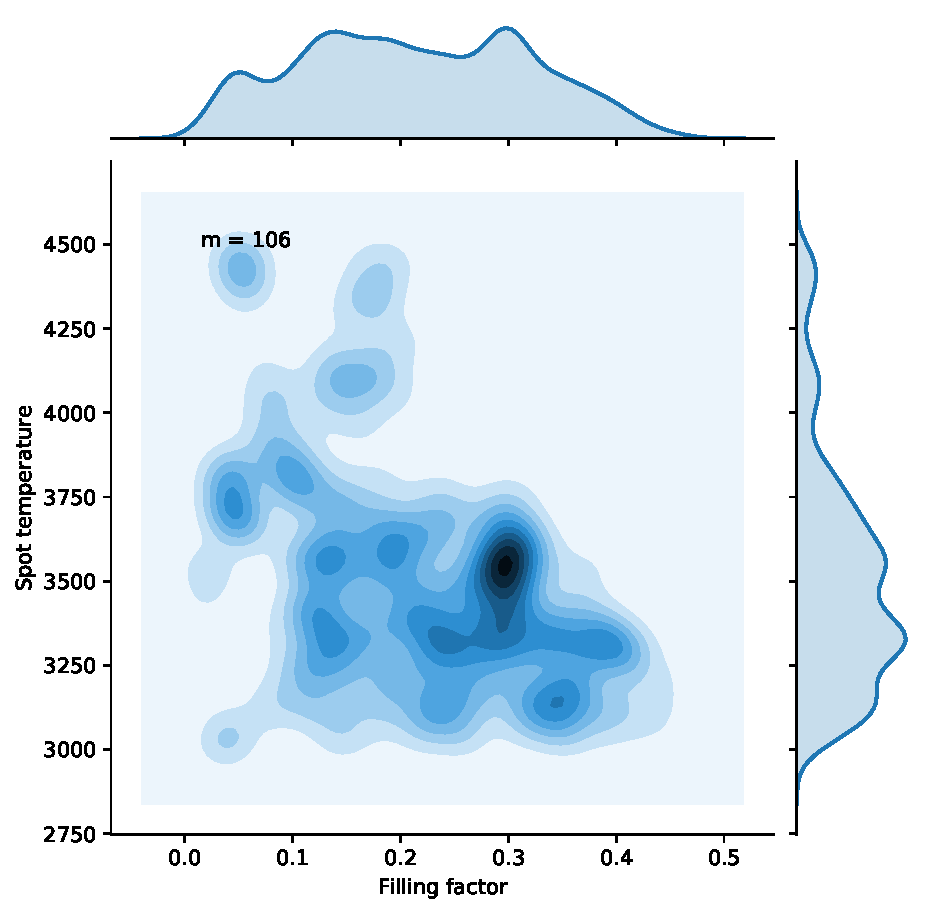
\includegraphics[width=2in]{figures/H_band_Tspot_fillingfactor_m106.pdf}}
   \end{tabular}
 \caption{2-dimensional distributions of filling factor and spot temperature for the nine accepted IGRINS orders for S1063. The median filling factor across these nine orders is $32 \pm 7$\% with a spot temperature of $4000\pm200$ K. As the IGRINS spectrum was observed at maximum light, these show a lower limit on the total spot coverage fraction. }
 \end{figure*}

\item What coverage fraction would we have measured across the rotational phase?
\end{itemize}

\section{Discussion}
\begin{itemize}
\item Spot coverage is consistent with formation theories
\item Conceivable geometries with circumpolar active longitudes, or migrating active latitudes
\item Biases introduced if we assume a spot-free model
\begin{itemize}
  \item Where does subsub sit in a new HR diagram? (new Somers models)
  \item *bonus* FIGURE: PMS HR diagram with new Somers tracks
  \item Spot impact on SED fits
\end{itemize}
\end{itemize}

\section{Conclusions}

Reiteration here.

\clearpage
\pagebreak


\appendix

\section{Are starspots confusing?}
\label{methods-details}

Short answer: no!

\acknowledgements

%ADS
We thank ADS!

%Kepler
This paper includes data collected by the Kepler mission. Funding for the Kepler mission is provided by the NASA Science Mission directorate.

% MAST
Some/all of the data presented in this paper were obtained from the Mikulski Archive for Space Telescopes (MAST). STScI is operated by the Association of Universities for Research in Astronomy, Inc., under NASA contract NAS5-26555.


{\it Facilities:} \facility{Smith (IGRINS)}, \facility{AAVSO}, \facility{INTEGRAL (OMC)}, \facility{ASAS}, \facility{Gaia}

{\it Software: }
 \project{pandas} \citep{mckinney10},
 \project{emcee} \citep{foreman13},
 \project{matplotlib} \citep{hunter07},
 \project{numpy} \citep{vanderwalt11},
 \project{scipy} \citep{jones01},
 \project{ipython} \citep{perez07},
 \project{gatspy} \citep{JakeVanderplas2015},
 \project{starfish} \citep{czekala15},
 \project{seaborn} \citep{waskom14}
%\software{%
% \project{pandas} \citep{mckinney10}
%    \project{emcee} \citep{foreman13},
% \project{matplotlib} \citep{hunter07},
% \project{numpy} \citep{vanderwalt11},
% \project{scipy} \citep{jones01},
% \project{ipython} \citep{perez07},
% \project{gatspy} \citep{JakeVanderplas2015},
% \project{starfish} \citep{czekala15}}.

\clearpage

\bibliographystyle{apj}
\bibliography{ms}

\end{document}
